\begin{figure}[h]
	\centering
	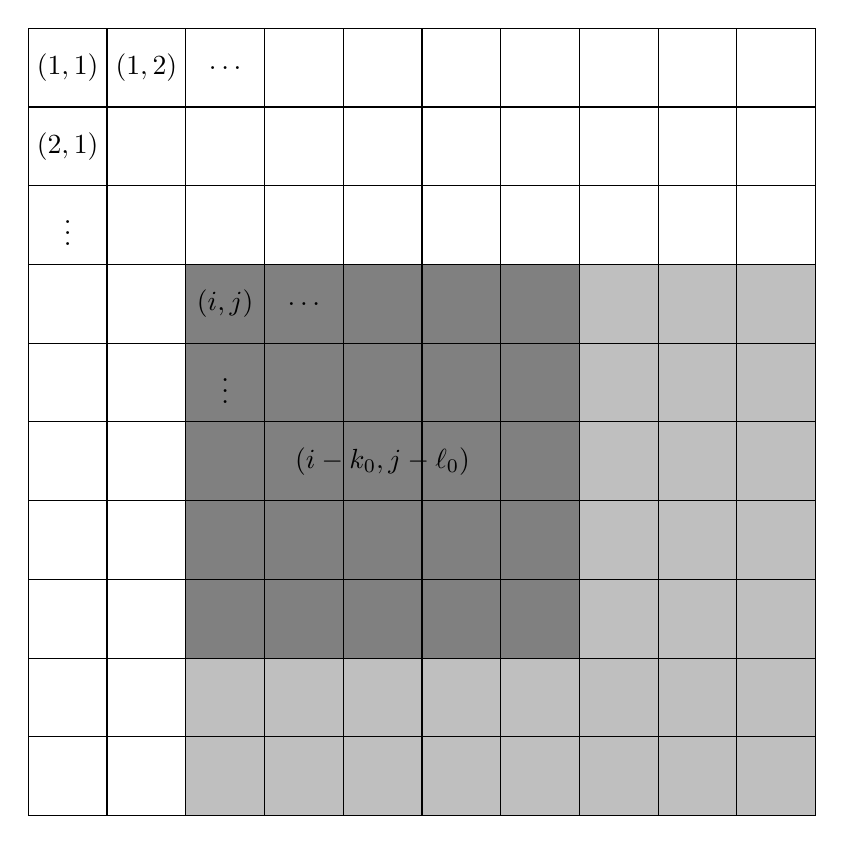
\begin{tikzpicture}
		\foreach \i in {-5, ..., 4}
			\foreach \j in {-5, ..., 4}
				\filldraw[white] (\i, \j) rectangle + (1, 1);
		\foreach \i in {-3, ..., 4}
			\foreach \j in {-5, ..., 1}
				\filldraw[gray, opacity=0.5] (\i, \j) rectangle + (1, 1);
		\foreach \i in {-3, ..., 1}
			\foreach \j in {-3, ..., 1}
				\filldraw[gray] (\i, \j) rectangle + (1, 1);
		\draw[step=1] (-5, -5) grid (5, 5);
		\node at (-2.5, 1.5) {$(i, j)$};
		\node at (-1.5, 1.5) {$\dots$};
		\node at (-2.5, 0.5) {$\vdots$};
		\node at (-0.5, -0.5) {$(i - k_0, j - \ell_0)$};
		\node at (-4.5, 4.5) {$(1, 1)$};
		\node at (-3.5, 4.5) {$(1, 2)$};
		\node at (-2.5, 4.5) {$\dots$};
		\node at (-4.5, 3.5) {$(2, 1)$};
		\node at (-4.5, 2.5) {$\vdots$};
	\end{tikzpicture}
	\caption{White pixels represent background, light gray pixels represent foreground. The indices $(k_0, \ell_0) \in \Psi_\varphi$ are chosen, such that for all $\tilde{k}, \tilde{\ell} \in \Phi_\varphi$ the pixels $(i - k_0 + \tilde{k}, j - \ell_0 + \tilde{\ell})$ belong to the foreground. These pixels are marked as dark gray.}
	\label{fig: setofforegroundpixels}
\end{figure}